% This tex file is available under a
% Creative Commons Attribution-Share Alike license (CC BY-SA 2.0).
% http://creativecommons.org/licenses/by-sa/2.0/
% Copyright © 2013 Rodrigo Hausen
\documentclass{beamer}
\usepackage[utf8]{inputenc}
\usepackage{lmodern}
\usepackage[T1]{fontenc}
\usepackage[portuguese,brazil]{babel}
\usepackage{url}
\usepackage{listings}
\usepackage{color}
\usepackage{textcomp}
\usepackage{pdfpages}
\usepackage{fancyvrb}
\usepackage{enumerate}
\usepackage{alltt}
%\usepackage[pdf]{pstricks}
%\usepackage{auto-pst-pdf}
%\usepackage{icomma} % para vírgula decimal / decimal comma
\definecolor{listinggray}{gray}{0.9}
\definecolor{mediumgray}{rgb}{0.6,0.6,0.6}
\definecolor{lbcolor}{rgb}{0.9,0.9,0.9}
\lstset{
    backgroundcolor=\color{lbcolor},
    tabsize=4,
    rulecolor=,
    basicstyle=\scriptsize,
    upquote=true,
    aboveskip={1.5\baselineskip},
    columns=fixed,
    showstringspaces=false,
    extendedchars=true,
    breaklines=true,
    prebreak = \raisebox{0ex}[0ex][0ex]{\ensuremath{\hookleftarrow}},
    frame=single,
    showtabs=false,
    showspaces=false,
    showstringspaces=false,
    identifierstyle=\ttfamily,
    keywordstyle=\color[rgb]{0,0,1},
    commentstyle=\color[rgb]{0.133,0.545,0.133},
    stringstyle=\color[rgb]{0.627,0.126,0.941},
}
\definecolor{pinegreen}{RGB}{0,139,114}
\definecolor{pgr}{RGB}{0,139,114}

\definecolor{aquamarine}{RGB}{0,181,190}
\definecolor{aqm}{RGB}{0,181,190}

\definecolor{skyblue}{RGB}{100,227,251}
\definecolor{skb}{RGB}{100,227,251}


\newcommand{\WD}[1]{\fbox{#1}\hspace{-0.5pt}}
\newcommand{\FWD}[1]{%
\fbox{%
\vbox to 10pt{\vfil%
\hbox to 0.8cm{\hfill#1\hfill}%
\vfil}%
}\hspace{-0.5pt}%
}

\def\A{\texttt{A}}
\def\B{\texttt{B}}
\def\C{\texttt{C}}
\def\D{\texttt{D}}
\def\E{\texttt{E}}
\def\F{\texttt{F}}

\usetheme{Boadilla}
%\usetheme{umbc2}
\usefonttheme{structuresmallcapsserif}
\usecolortheme{seahorse}

\title{Aula 8: Portas Lógicas}
\subtitle{Circuitos Digitais}
\author{Rodrigo Hausen}
\institute{CMCC -- UFABC} 
\date{21 de fevereiro de 2013}

\begin{document}

\begin{frame}
\maketitle

\vspace{-1cm}

\begin{center}
\url{http://compscinet.org/circuitos}
\end{center}

\end{frame}

%%%%%%%%%%%%%%%%%%%%%%%%%%%%%%%%%%%%%%%%%%%%%%%%%

\begin{frame}
\frametitle{Controlando um interruptor com sinal elétrico}

\begin{itemize}
\item Solução para a pergunta 2a: use um eletroíma!
\end{itemize}

\only<1>{%
\centering%
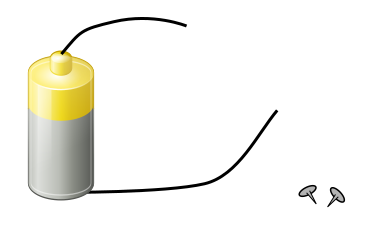
\includegraphics{images/magneto1.png}%
}%
\only<2>{%
\centering%
\includegraphics{images/magneto2.png}%
}%
\only<3>{%
\centering%
\includegraphics{images/magneto3.png}%
}
\only<4>{%
\centering%
\includegraphics{images/magneto4.png}%
}

\end{frame}

\begin{frame}
\frametitle{Relé}

\begin{itemize}
\item Relé: componente eletromecânico composto por um eletroíma e um interruptor
\end{itemize}

Relé normalmente fechado (NF):

\centering%
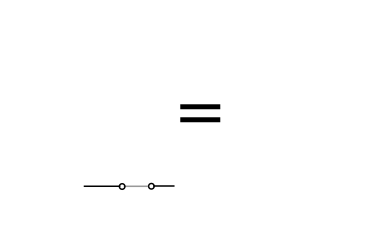
\includegraphics{images/magneto5}%

\end{frame}

\end{document}
